\documentclass[10pt,conference,compsocconf]{IEEEtran}

%\usepackage{times}
%\usepackage{balance}
\usepackage{url}
\usepackage{graphicx}	% For figure environment
\usepackage{color}
\usepackage{amsmath}

\begin{document}
\title{Applying WaveNet on frequency data}

\author{
  Luzi Sennhauser\\
  Christoph Dehner\\
  Department of Computer Science, ETH Zurich, Switzerland
}

\maketitle

\begin{abstract}
  A critical part of scientific discovery is the
  communication of research findings to peers or the general public.
  Mastery of the process of scientific communication improves the
  visibility and impact of research. While this guide is a necessary
  tool for learning how to write in a manner suitable for publication
  at a scientific venue, it is by no means sufficient, on its own, to
  make its reader an accomplished writer. We also describe the rules
  for submission in the computational intelligence laboratory.
  This guide should be a
  starting point for further development of writing skills.
\end{abstract}

\section{Introduction}
In 2016, \cite{wavenet} introduced WaveNet, a generative model for raw audio achieving astonishing results in learning sound features and generating smooth audio. Trained on piano music, new highly dynamic piano music varying in melody, volume and speed smoothly could be generated.\\
The aim this paper is to enhance the WaveNet architecture and apply it to a more feature-oriented representation of input data. Instead of performing a classification task on raw audio, the network is adopted to operate on the frequencies of the audio data, processed by Fouier transformation. In particular, the following topics are covered:
\begin{itemize}
\item Based on WaveNet from \cite{wavenet} a network architecture to generate music is introduced operating on the frequencies of audio input.
\item This new network is trained and evaluated on piano music from the MusicNet dataset. Furthermore, optimization approaches as data normalization and variations in preprocessing the data are included in the experiments.
\item Results from the evaluation are analyzed in detail. In the context of the introduced network, advantages as well as weaknesses are discussed. 
\end{itemize}
As training data in the experiments, piano samples from the MusicNet dataset, a collection of 330 freely-licenced recordings of classical music are taken. The data is publicly available online \cite{musicnet}.\\
The source code of the experiments can be found on GitHub.\footnote{\url{https://github.com/sennluzi/tensorflow-wavenet}}

\section{Models and Methods}
The following section describes the underlying model of the network used in the experiments of this paper. As core network the WaveNet architecture with a stack of dilated causal convolutional layers (figure \ref{fig:wavenet_dilated_cnn}) is taken. Hereupon, the data input layer is changed conceptually.
\begin{figure}[tbp]
  \centering
  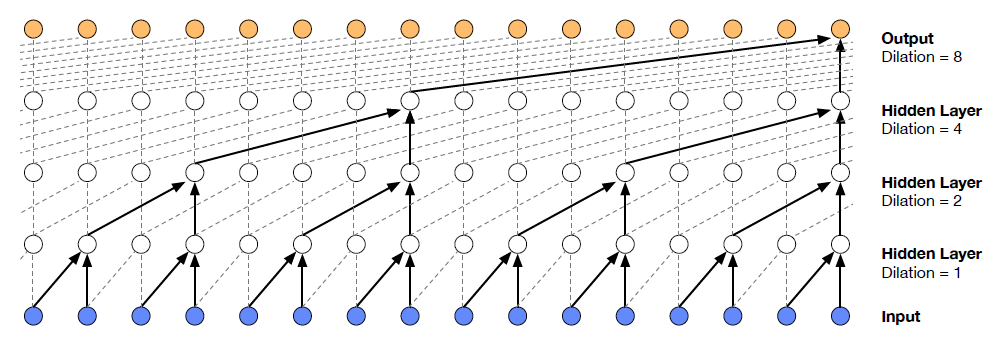
\includegraphics[width=\columnwidth]{figures/wavenet_dilated_cnn.png}
  \caption{dilated convolutional network}
  \label{fig:wavenet_dilated_cnn}
\end{figure}

\subsection{WaveNet architecture}
Given a sequence of amplitudes, WaveNet predicts the subsequent amplitude. The amplitudes are quantized in 256 bins \cite{itu1988711}. In the $i$th step, the network then outputs a probability distribution $P(x_{i+1} | x_1, ..., x_i)$. The amplitude $x_{i+1}$ of the next step is then sampled according to that distribution.\\
In WaveNet, training can be done in parallel while the generation of a audio sample is done sequentially.\\
As a basis for WaveNet, the implementation of Igor Babuschkin is taken \cite{Babuschkin2016}.\\
The original WaveNet paper mentiones only very few coefficients for how their network is configured. Therefore reproducing the paper exactly is very hard. The following numbers are assumptions mainly based on the experience of Babuschkin's implementation. In the following experiments, the dilations are $2^n$ for $n$ taking the values $(0,1,...,7,8)$ and are repeated 5 times. This leads to 50 hidden dilation layers. The convolution filter size is set to $2$ and the number of channels of the residual and the dilation is $32$.\\
The input of the WaveNet network is a sequence of amplitudes, each of which encoded as a one-hot vector.

\textcolor{red}{rough description of wavenet architecture and specification used during the experiments}
\subsection{Data preprocessing}
To extract frequencies, the raw audio data consisting of pressure measurements are divided into chunks of size 2048, which are then transformed into the frequency space using FFT. Therefrom, the first 150 coefficients are taken as dominant frequencies for the subsequent training. To ensure that audio features are transformed smoothly, two neighboring raw audio chunks overlap in a few samples, described by a variable $stride$. Equation \ref{eq:fft} summarized the frequency extraction of the $i^\textnormal{th}$ chunk compactly.
\begin{multline}\label{eq:fft}
\textnormal{frequencies\_coeffs}_i =
FFT(\textnormal{inputData}[i \cdot stride:\\i \cdot stride+2048])[:150]
\end{multline}
Considering real and imaginary parts of the complex Fourier coefficients separately, each chunk of 2048 raw audio samples is transformed into 300 real frequency values.\\
To decrease the dimensionality even further, principle component analysis (PCA) is used to reduce these 300 frequencies to 100 values.
These 100 PCA coefficient are considered one tone and fed into the network as one time step.\\
The eigenvectors of the PCA are shown in figure \ref{fig:pca_eigenvectors_imaginary_numbers}. Figure \ref{fig:pca_eigenvectors} illustrates how the PCA looks like when taking the absolute values of the imaginary numbers, out of which the components are built from. In this figure, one can see, that the relevant frequencies are all relatively low. Figure \ref{fig:pca_explained_variance} shows that a vast majority of the variance of the frequencies is captured by the first 100 PCA components. Summarizing, in neither of the two steps, we loose much of the original input information. This should lead to a decent compression of the audio signal.\\
To make this evident, one can figure invert all the steps and plot the compressed wave and the original wave (see \ref{fig:preprocessing_difference_waveform}). It is easy to see that they resemble a lot. After preprocessing the audio contains a cracking noise, but nevertheless is the melody and the tone of the music well audible.\\
To ensure this preprocessing still preserves the nature of the music, one can invert all steps. Although after preprocessing, there is an audible cracking, the music then is still clearly hearable and the pitches recognizable.
On one hand, the waveform looks still similar (figure \ref{fig:preprocessing_difference_waveform})
Whereas in the original WaveNet architecture, 16000 samples represented on second of audio, the adopted network only needs to process $16000/2048 \approx 8$ samples per second. However, this change infers a fundamentally different approach of audio training and generation, described in the next section. 

\begin{figure}[tbp]
  \centering
  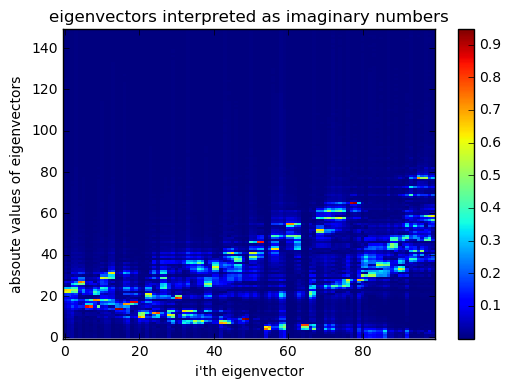
\includegraphics[width=\columnwidth]{figures/pca_eigenvectors_imaginary_numbers.png}
  \caption{Eigenvectors of the PCA where the imaginary and the real part of the FFT are stored as a separate value in the PCA component.}
  \label{fig:pca_eigenvectors_imaginary_numbers}
\end{figure}

\begin{figure}[tbp]
  \centering
  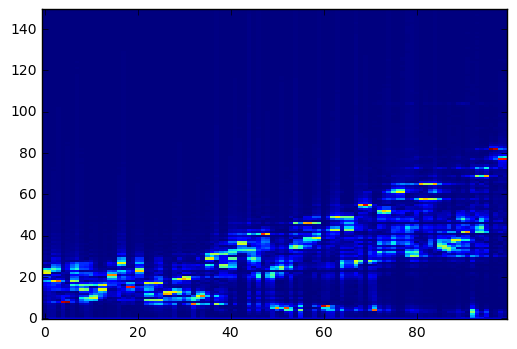
\includegraphics[width=\columnwidth]{figures/pca_eigenvectors.png}
  \caption{Transformed eigenvectors of the PCA: The values of the vectors are the absolute value of the corresponding imaginary number}
  \label{fig:pca_eigenvectors}
\end{figure}

\begin{figure}[htbp]
  \centering
  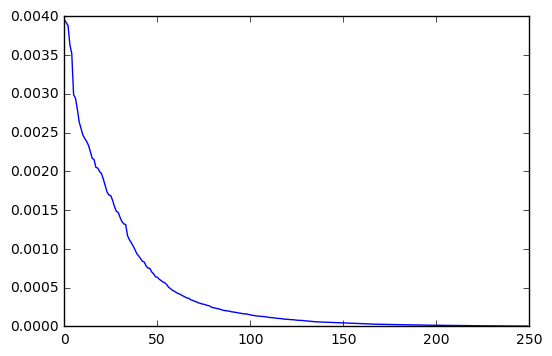
\includegraphics[width=\columnwidth]{figures/pca_explained_variance}
  \caption{Signal compression and denoising using the Daubechies wavelet basis.}
  \label{fig:pca_explained_variance}
\end{figure}

\begin{figure}[tbp]
  \centering
  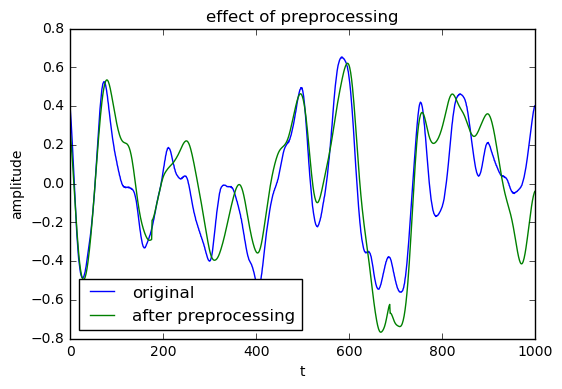
\includegraphics[width=\columnwidth]{figures/preprocessing_difference_waveform}
  \caption{An example of how the output audio differs before and after preprocessing (compression)}
  \label{fig:preprocessing_difference_waveform}
\end{figure}

\subsection{Network architecture and loss}
Whereas the original WaveNet paper designed the network to perform a classification task, the adopted network aims to train and predict the frequencies of a audio sample directly. The network input during one time step is now not only one class describing the current tone, but a 100 dimensional vector representing the frequencies of the tone of time step in a compressed way. Similarly, the output of the network is no longer a softmax layer but also a 100 dimensional vector.\\
This change in architecture also affects the loss during training. Instead of a softmax cross-entropy loss the adopted network uses the mean squared error as loss function during training.

\section{Results}
The generated audio files start with some fastly changing frequencies and then after 30-40 frames (1-2 seconds) it stabilizes on one distribution of frequencies. From then on the values of the frequencies do not change any more. Figures \ref{fig:original_frequencies} and \ref{fig:generated_frequencies} show that the neural network is not able to produce a change of frequencies while a real piece of music observes a change every 20-200 frames.\\
The consequence of these frequencies not changing is, that the audio file consists after a noise at the beginning only of a steady pitch. And it doesn't resemble a pitch either.\\

\begin{figure}[tbp]
  \centering
  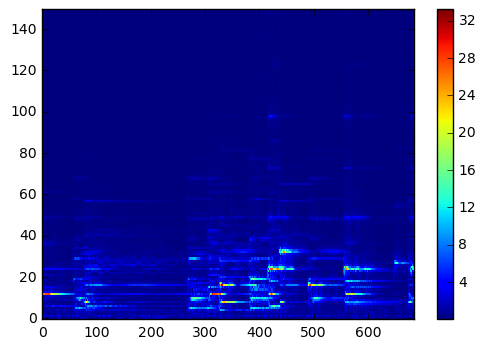
\includegraphics[width=\columnwidth]{figures/original_frequencies.png}
  \caption{Frequencies of a piano piece used for training}
  \label{fig:original_frequencies}
\end{figure}
\begin{figure}[tbp]
  \centering
  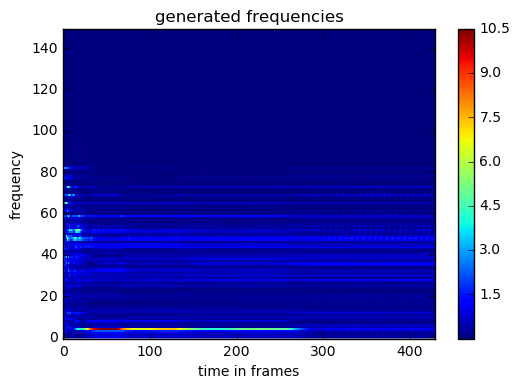
\includegraphics[width=\columnwidth]{figures/generated_frequencies_20s.png}
  \caption{Frequencies of the generated audio piece}
  \label{fig:generated_frequencies}
\end{figure}

\begin{figure*}[tbp]
  \centering
  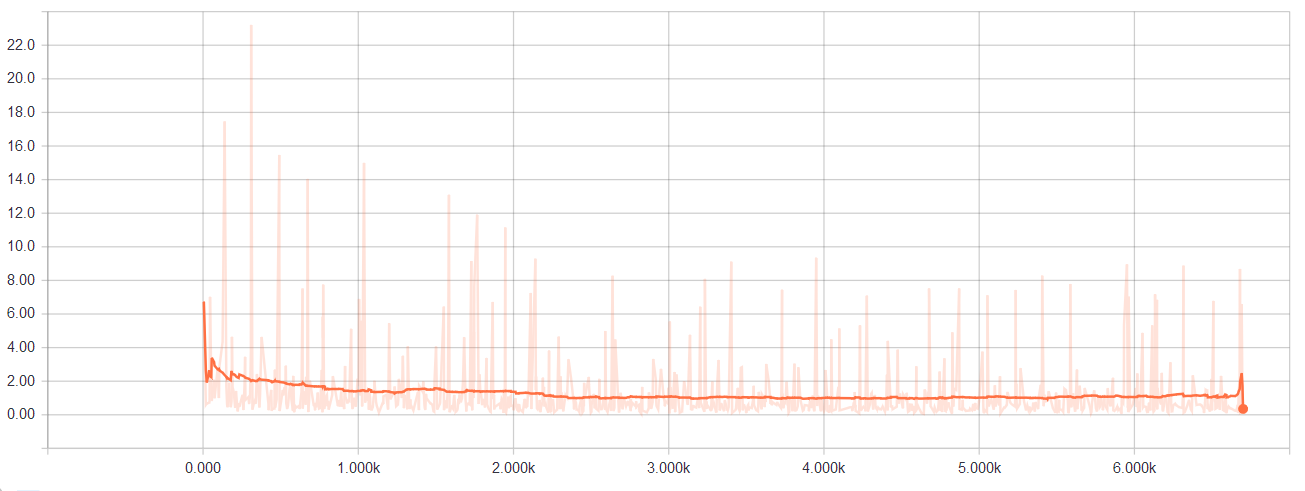
\includegraphics[width=\textwidth]{figures/loss.png}
  \caption{Training error}
  \label{fig:training_error}
\end{figure*}

\section{Discussion}
The approach of this paper could be promising due to the following reason: The original WaveNet paper's network has to learn the behaviour of sound consisting of repetitive oscillations. With transforming the signal to the Fourier space, we take this burden from the neural network. The network can focus on data which is more related to the final tone. For example when a tone is repeated for 1s, this is also the same output of the network.\\
But it might be exactly this phenomenon which makes good music generation impossible. During training, the network might do really well only staying on one and the same pitch, because changes happen in too rare occasions to influence the overall loss.\\
When improving this approach further, one could try to include the rate of changing tones into the loss function and to punish a network when producing too many times in a row a similar output.\\

\section{Summary}


\bibliographystyle{IEEEtran}
\bibliography{paper}
\end{document}
